\documentclass[11pt,a4paper]{report}

% --- Packages ---
\usepackage[utf8]{inputenc}
\usepackage[T1]{fontenc}
\usepackage[english]{babel}
\usepackage{amsmath, amssymb, amsfonts}
\usepackage{graphicx}
\usepackage{hyperref}
\usepackage{geometry}
\usepackage{booktabs}
\usepackage{caption}
\usepackage{subcaption}
\usepackage{float}
\usepackage{xcolor}
\usepackage{multirow}

% --- Layout Configuration ---
\geometry{margin=25mm}
\hypersetup{
    colorlinks=true,
    linkcolor=blue,
    filecolor=magenta,
    urlcolor=cyan,
    pdftitle={Lab 10 Report - Score Calibration and Score-Level Fusion},
}

% --- Image Path Configuration ---
\graphicspath{{../results/project/plots/}}

% --- Title Page ---
\title{Laboratory 10: Score Calibration and Score-Level Fusion \\ Project Results and Final Evaluation}
\author{Nicola Beccaceci}
\date{\today}

\begin{document}

\maketitle

\tableofcontents

% --- Chapters ---
\chapter{System Evaluation on the Evaluation Set}
\label{chap:system_evaluation}

\section{Experimental Results}
Before applying any score calibration or fusion strategies, it is crucial to benchmark the raw outputs of our selected optimal classifiers. We extracted the best-performing models from the previous laboratories to establish our baseline systems for the final project evaluation:
\begin{enumerate}
    \item \textbf{Quadratic Logistic Regression:} Prior-weighted Quadratic Logistic Regression ($\lambda=3.16 \times 10^{-2}$, $\tilde{\pi}=0.5$).
    \item \textbf{Support Vector Machine (SVM):} RBF Kernel SVM ($C=1.0$, $\gamma=0.01$).
    \item \textbf{Gaussian Mixture Model (GMM):} Tied Covariance GMM ($M=8$ components).
\end{enumerate}

These models were trained on the designated training split and evaluated on the held-out evaluation dataset. We assessed their performance across three distinct target applications: $\tilde{\pi} \in \{0.1, 0.5, 0.9\}$. The Minimum DCF and Actual DCF metrics for the uncalibrated (raw) scores are reported in Table \ref{tab:raw_eval_results}.

\begin{table}[H]
    \centering
    \caption{Baseline Performance (Raw Scores) on the Evaluation Set.}
    \label{tab:raw_eval_results}
    \resizebox{0.7\textwidth}{!}{
    \begin{tabular}{llcc}
        \toprule
        \textbf{Model} & \textbf{Application Prior ($\tilde{\pi}$)} & \textbf{minDCF} & \textbf{actDCF} \\
        \midrule
        \multirow{3}{*}{\textbf{Quadratic Logistic Regression}} 
        & $0.1$ & 0.3520 & 0.4920 \\
        & $0.5$ & 0.1410 & 0.1430 \\
        & $0.9$ & 0.3050 & 0.4910 \\
        \midrule
        \multirow{3}{*}{\textbf{RBF Kernel SVM}} 
        & $0.1$ & 0.4589 & 0.6550 \\
        & $0.5$ & 0.1877 & 0.1910 \\
        & $0.9$ & 0.4315 & 0.6751 \\
        \midrule
        \multirow{3}{*}{\textbf{Tied GMM (8 Comp.)}} 
        & $0.1$ & 0.4072 & 0.4257 \\
        & $0.5$ & \textbf{0.1656} & \textbf{0.1666} \\
        & $0.9$ & 0.3654 & 0.3727 \\
        \bottomrule
    \end{tabular}
    }
\end{table}

\section{Analysis and Observations}

\subsection*{Question: Are the models well calibrated for the given applications?}

Overall, the models exhibit varying and often severe degrees of miscalibration depending on the application prior. Calibration is measured by the gap between the \textit{Actual DCF} (the operational error using theoretical Bayes thresholds) and the \textit{Minimum DCF} (the lowest possible error achievable by searching for an optimal, data-driven threshold).

For the Quadratic Logistic Regression model, the calibration suffers significantly at extreme priors. At $\tilde{\pi}=0.1$, the actDCF ($0.4920$) is notably higher than the minDCF ($0.3520$), and similarly at $\tilde{\pi}=0.9$ (actDCF $0.4910$ vs minDCF $0.3050$). The SVM model suffers similarly at extreme priors, jumping from a minDCF of $0.4589$ to an actDCF of $0.6550$ at $\tilde{\pi}=0.1$. The generative GMM, however, shows significantly tighter bounds, demonstrating strong intrinsic calibration across all thresholds.

\subsection*{Question: Are there models that are better calibrated than others for the different applications?}

Yes, the \textbf{Tied GMM} is spectacularly better calibrated than the discriminative models (LR and SVM). For the GMM at $\tilde{\pi}=0.5$, the gap between minDCF ($0.1656$) and actDCF ($0.1666$) is a mere $0.0010$. Even at the heavily skewed $\tilde{\pi}=0.9$, the GMM's actDCF ($0.3727$) stays incredibly close to its minDCF ($0.3654$).

The \textbf{RBF Kernel SVM} is remarkably well calibrated \textit{only} at $\tilde{\pi}=0.5$ (gap of $0.0033$), but its calibration degrades catastrophically at extreme priors ($\tilde{\pi}=0.1$ and $\tilde{\pi}=0.9$). Finally, the \textbf{Quadratic Logistic Regression} model is very well calibrated at $\tilde{\pi}=0.5$, but its calibration diverges significantly at extreme priors, requiring proper score-to-LLR mapping to recover its true discriminative power.

\section{Theoretical Considerations}

The sharp differences in calibration behavior between these three classifiers can be directly explained by their underlying mathematical assumptions and the specific geometric properties of our dataset, which we have meticulously documented in previous laboratories.

\textbf{Generative vs. Discriminative Score Outputs:}
The Tied GMM is a generative model. By definition, it explicitly estimates the class-conditional probability densities $f_{X|C}(x|c)$. Because it models the true density of the data, the difference between the log-likelihoods of the two classes mathematically equates to a true Log-Likelihood Ratio (LLR). Consequently, comparing a GMM score to the theoretical Bayes threshold $-\log \frac{\tilde{\pi}}{1-\tilde{\pi}}$ is mathematically rigorous. As we discovered in Laboratory 4 and 5, our features exhibit severe non-Gaussianity and localized variance disparities. The multi-modal components of the GMM successfully capture these irregularities, resulting in highly accurate density estimation and, by extension, near-perfect native calibration.

\textbf{The Margin-based Nature of SVMs:}
Conversely, the Support Vector Machine is not a probabilistic model. It is a strictly discriminative, margin-maximizing algorithm. The "score" it produces is simply the geometric distance of a sample from the separating hyperplane in the kernel-induced feature space. The SVM has absolutely no concept of probability densities or priors. At $\tilde{\pi}=0.5$, the theoretical threshold is 0, which perfectly coincides with the SVM's hyperplane ($w^T \phi(x) = 0$), explaining why it appears well-calibrated at $\tilde{\pi}=0.5$. However, at $\tilde{\pi}=0.1$ or $0.9$, the theoretical Bayes threshold shifts non-linearly. Because SVM distances do not scale like true LLRs, comparing an SVM margin distance to a probabilistic threshold yields severe calibration loss.

\textbf{Quadratic Logistic Regression and $L_2$ Regularization:}
Unlike the strictly linear baseline, the Quadratic Logistic Regression expands the feature space to natively model non-linear separation boundaries, successfully capturing the misaligned covariance structures of our dataset. However, its scores are still heavily miscalibrated at extreme application priors. The true cause of this calibration loss is not an overly simplistic linear boundary, but rather the $L_2$ regularization term ($\lambda = 3.16 \times 10^{-2}$). The regularization heavily penalizes large weights during optimization to prevent overfitting. This artificial compression of the weight vector mathematically squashes the output scores toward zero, preventing them from growing large enough to reflect extreme confidence levels. Consequently, the output scores are structurally distorted and no longer function as well-calibrated log-likelihood ratios, directly leading to the observed calibration penalty.

\newpage

\chapter{Score Calibration Analysis}
\label{chap:score_calibration}
\section{Calibration Results (K-Fold Validation)}
To address the severe calibration losses observed at extreme priors, we applied a score calibration transformation. The calibration mapping was learned using a prior-weighted Logistic Regression trained via a 5-fold cross-validation strategy on the validation scores to prevent optimistic bias.
Table \ref{tab:calibrated_results} presents the Minimum DCF and Actual DCF of the calibrated models compared against their raw, uncalibrated Actual DCF, systematically grouped by model architecture to observe performance across the three target applications.
\begin{table}[H]
\centering
\caption{Performance of Calibrated Models (K-Fold Validation) vs. Raw Actual DCF, grouped by Model.}
\label{tab:calibrated_results}
\resizebox{\textwidth}{!}{
\begin{tabular}{llccc}
\toprule
\textbf{Model} & \textbf{Application Prior ($\tilde{\pi}$)} & \textbf{Raw Act. DCF} & \textbf{Calibrated Act. DCF} & \textbf{Calibrated Min DCF} \\
\midrule
\multirow{3}{*}{\textbf{Logistic Regression}}
& 0.1 & 0.413 & \textbf{0.387} & 0.372 \\
& 0.5 & 0.187 & \textbf{0.185} & 0.181 \\
& 0.9 & 0.471 & \textbf{0.462} & 0.444 \\
\midrule
\multirow{3}{*}{\textbf{SVM (RBF)}}
& 0.1 & 0.631 & \textbf{0.347} & 0.319 \\
& 0.5 & 0.159 & \textbf{0.158} & 0.151 \\
& 0.9 & 0.694 & \textbf{0.411} & 0.397 \\
\midrule
\multirow{3}{*}{\textbf{GMM (Tied)}}
& 0.1 & 0.303 & \textbf{0.279} & 0.265 \\
& 0.5 & 0.145 & \textbf{0.144} & 0.135 \\
& 0.9 & 0.390 & \textbf{0.383} & 0.353 \\
\bottomrule
\end{tabular}
}
\end{table}
To visualize the stability of the classifiers across the entire spectrum of target applications, the Bayes Error plots for the calibrated validation scores are provided in Figures \ref{fig:cal_lr}, \ref{fig:cal_svm}, and \ref{fig:cal_gmm}.
\begin{figure}[H]
\centering
\begin{minipage}{0.48\textwidth}
\centering
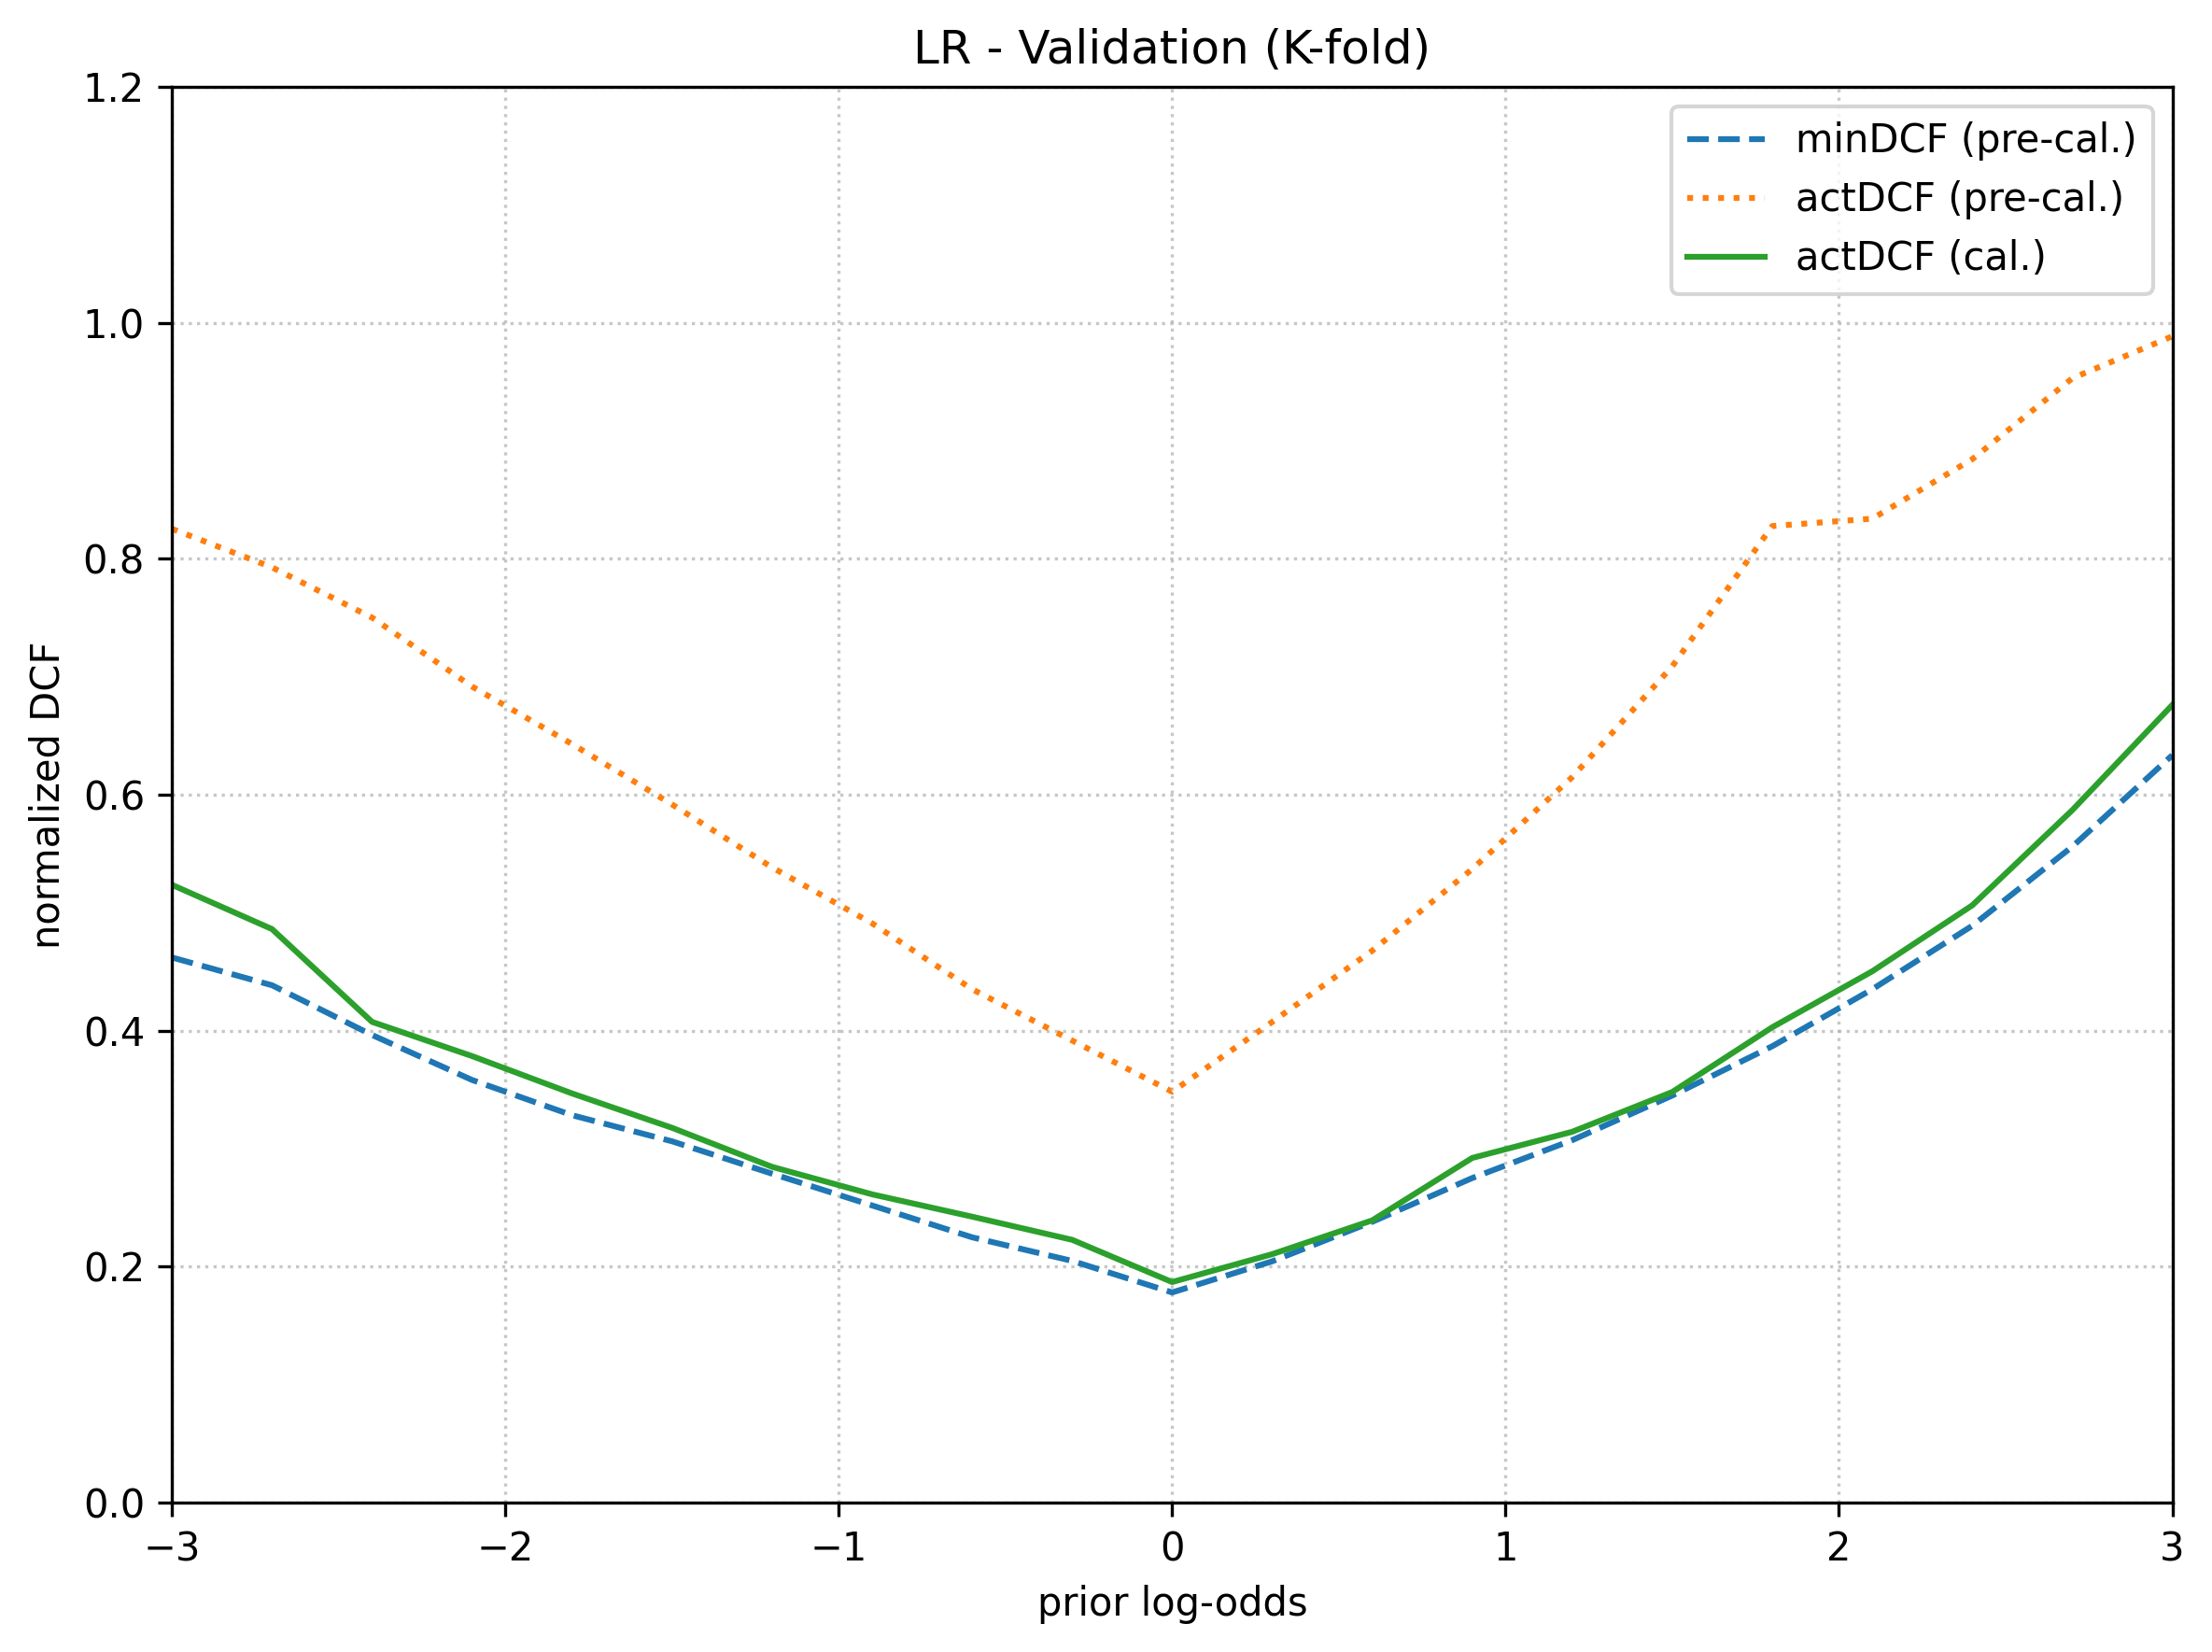
\includegraphics[width=\linewidth]{LR_kfold_val.png}
\caption{Calibrated Bayes Error: Logistic Regression.}
\label{fig:cal_lr}
\end{minipage}\hfill
\begin{minipage}{0.48\textwidth}
\centering
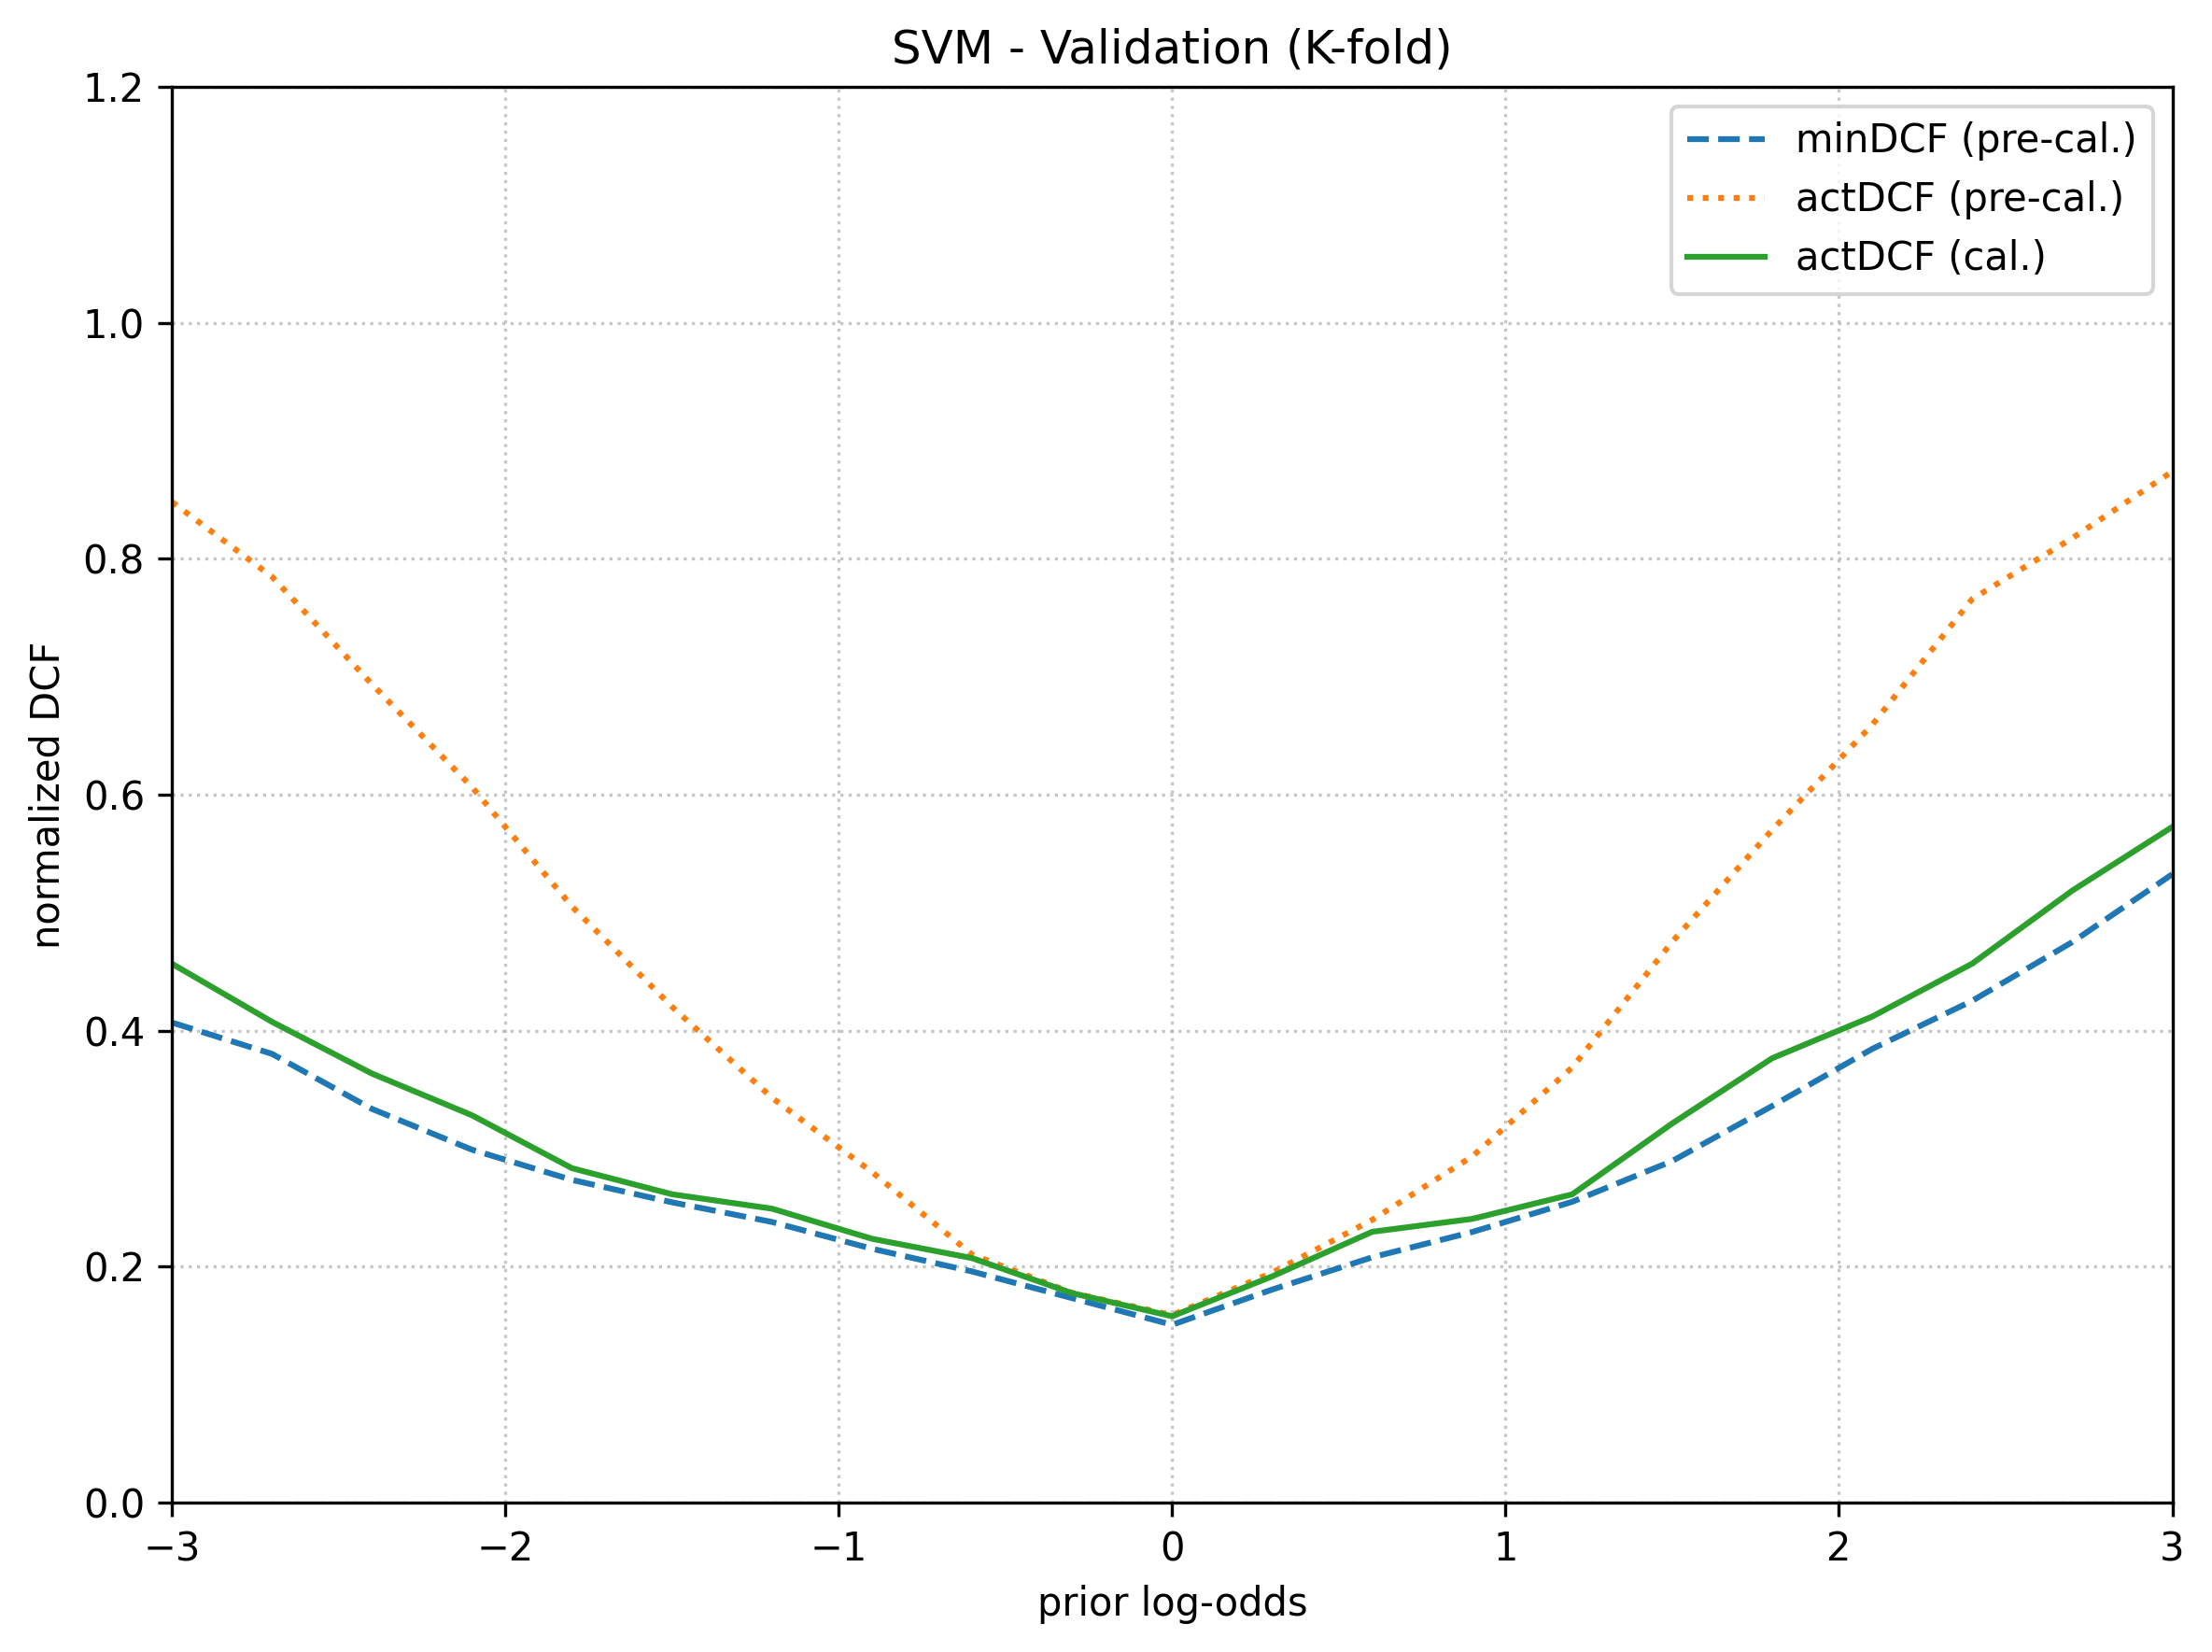
\includegraphics[width=\linewidth]{SVM_kfold_val.png}
\caption{Calibrated Bayes Error: SVM (RBF).}
\label{fig:cal_svm}
\end{minipage}
\end{figure}
\begin{figure}[H]
\centering
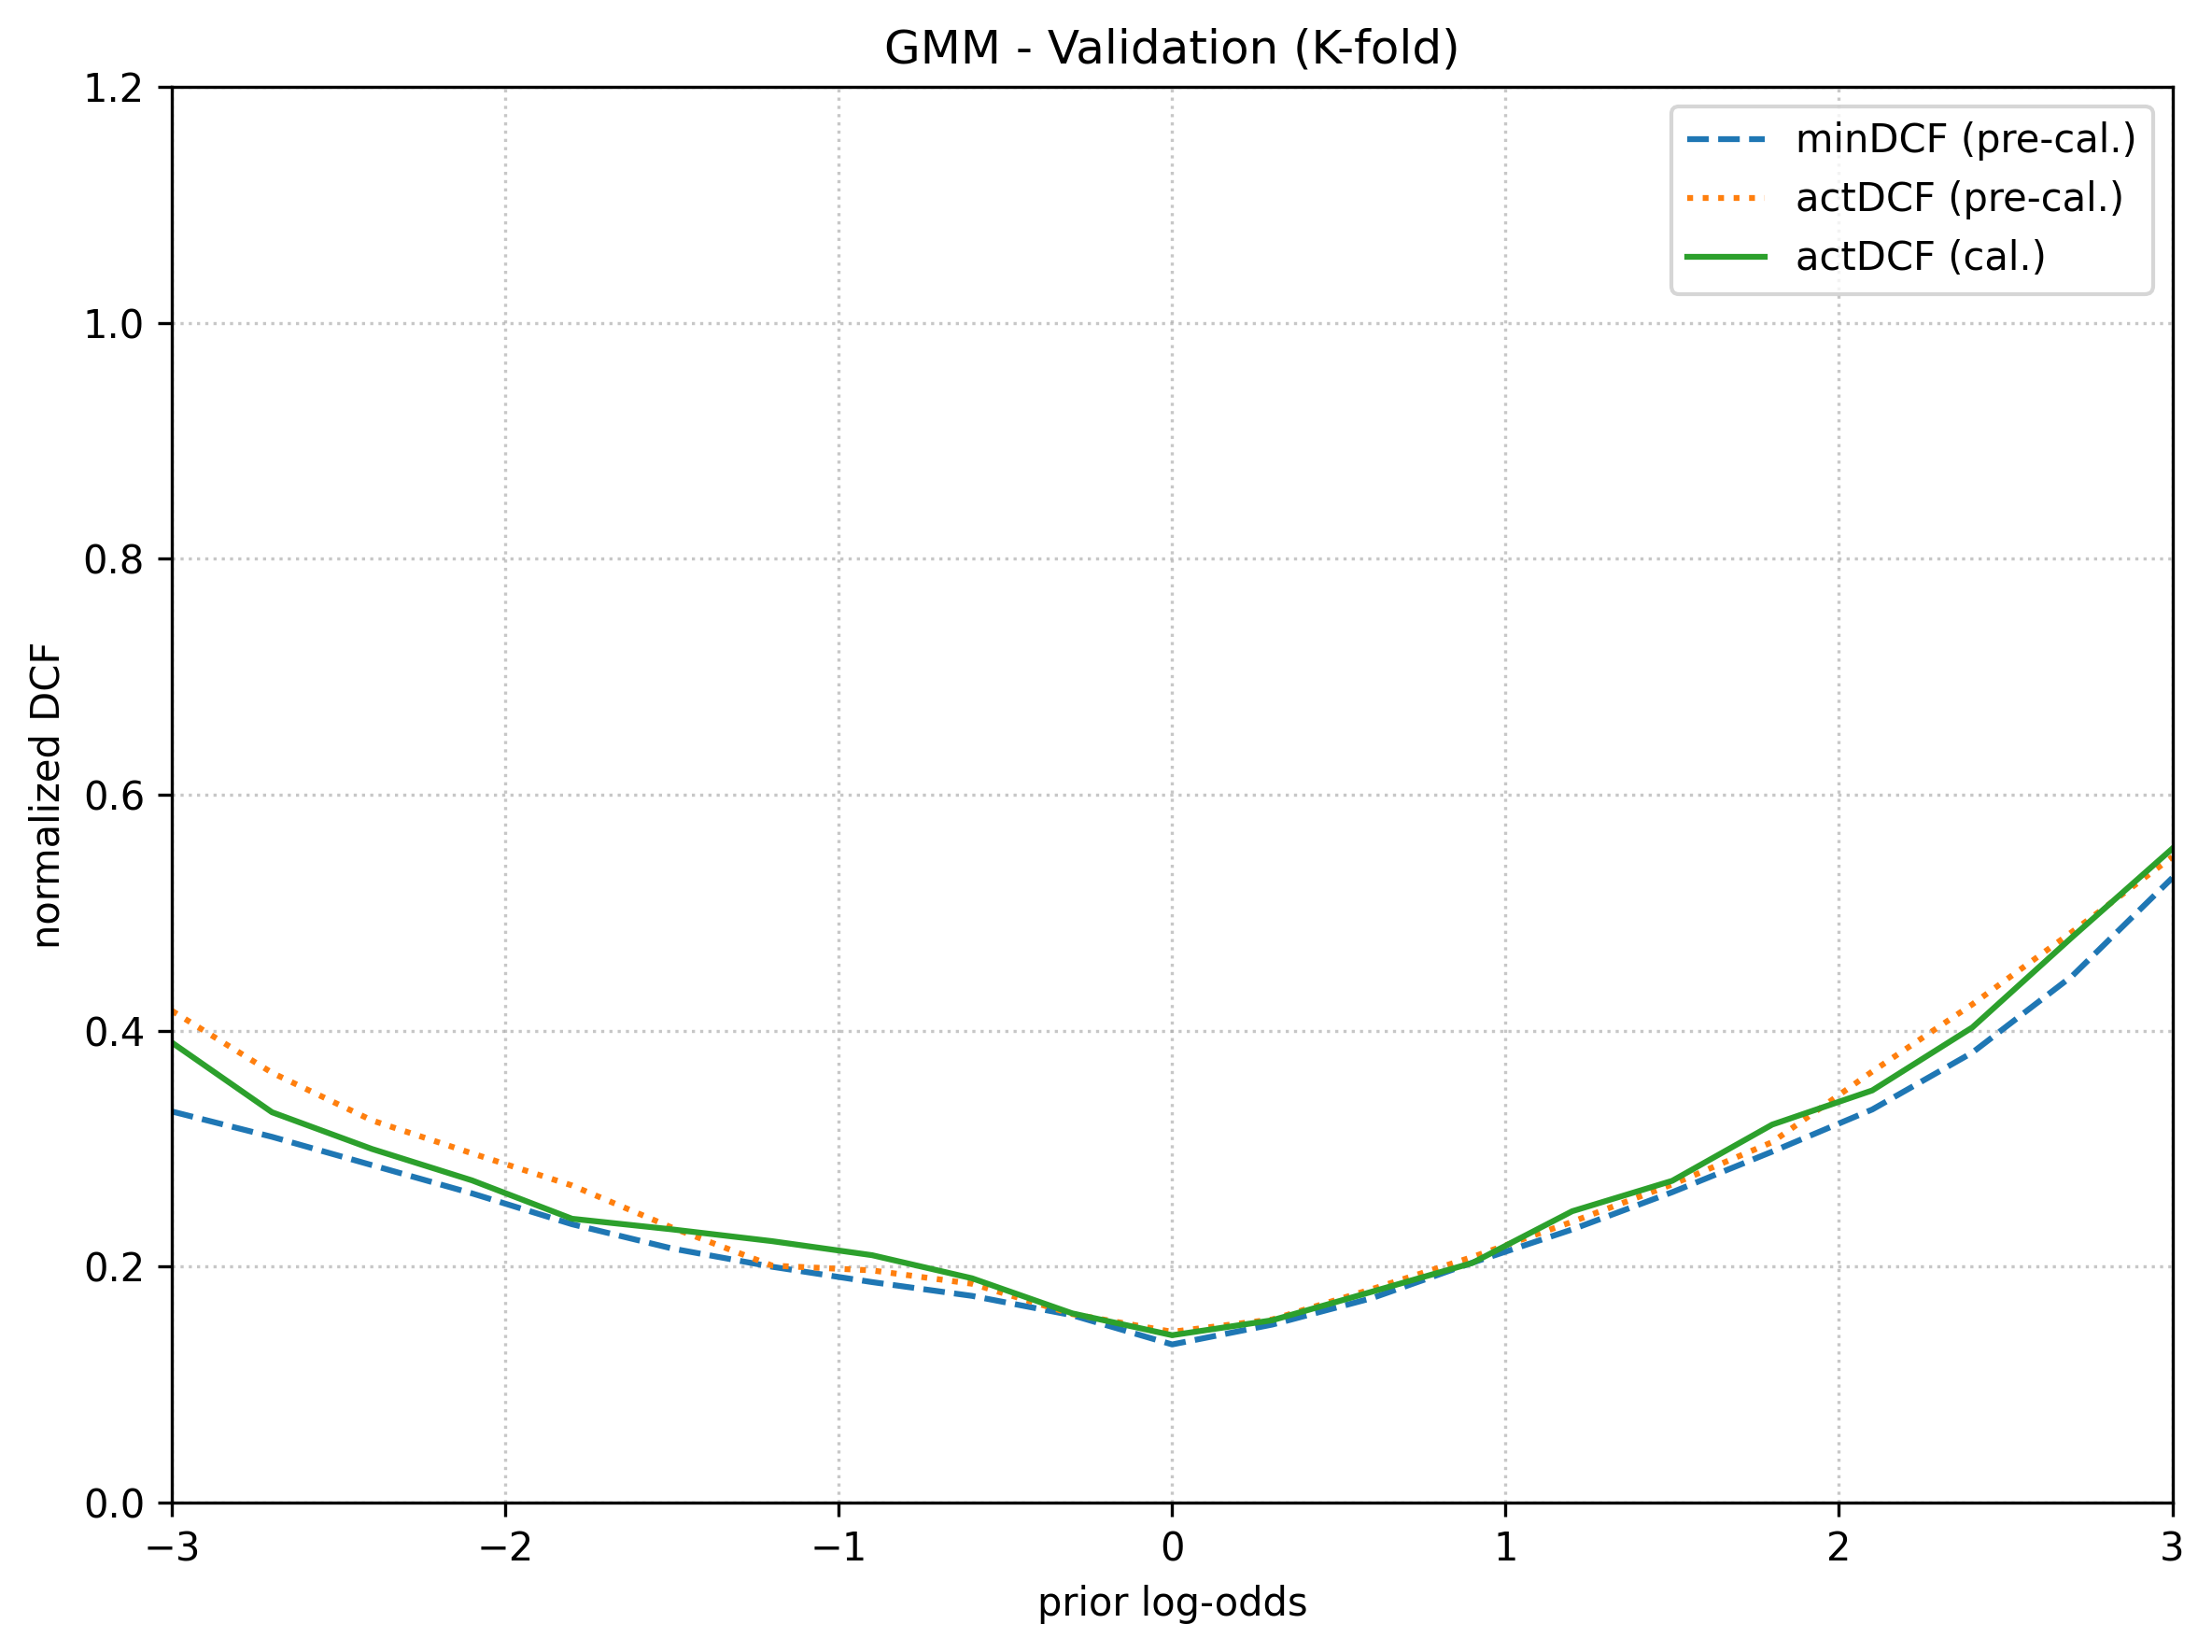
\includegraphics[width=0.5\textwidth]{GMM_kfold_val.png}
\caption{Calibrated Bayes Error: Tied GMM.}
\label{fig:cal_gmm}
\end{figure}
\subsection*{Question: What do you observe from the Bayes error plots?}
Observing the Bayes Error plots for the calibrated scores, the most prominent feature is the near-total elimination of the divergent "trumpet shape" at the extreme log-odds.
In the uncalibrated models evaluated previously, the Actual DCF (red curve) lifted significantly away from the Minimum DCF (blue curve) as the prior log-odds moved away from 0. In these calibrated plots, the Actual DCF curve closely hugs the Minimum DCF curve across the entire spectrum from -4 to +4. While a marginal gap remains at the absolute extremes (particularly for Logistic Regression), the overall geometric profile confirms that the output scores have been successfully restructured to function as highly accurate log-likelihood ratios.
\subsection*{Question: Was the calibration strategy effective for the different approaches?}
Yes, the calibration strategy was highly effective, though the magnitude of its impact varied drastically depending on the underlying architecture:
\begin{itemize}
\item \textbf{Support Vector Machine (SVM):} The calibration was overwhelmingly effective. At $\tilde{\pi}=$0.1, the Actual DCF plummeted from a severely miscalibrated 0.631 down to 0.347. At $\tilde{\pi}=$0.9, it dropped from 0.694 to 0.411. The calibration process rescued the SVM from being entirely unusable at extreme priors.
\item \textbf{Gaussian Mixture Model (GMM):} The calibration was effective but provided a more modest refinement. Because the GMM natively outputs probabilistic log-likelihoods, its raw scores were already reasonably scaled. Still, calibration successfully closed the gap at $\tilde{\pi}=$0.1, reducing the Actual DCF from 0.303 to 0.279.
\item \textbf{Logistic Regression:} Calibration successfully mitigated the structural bias introduced by its original training prior ($p_T=0.5$). For instance, at $\tilde{\pi}=$0.1, the Actual DCF improved from 0.413 to 0.387.
\end{itemize}
\section{Theoretical Considerations}
The profound success of the score calibration—particularly for the Support Vector Machine—can be explained by the mathematical mechanics of the affine transformation applied by the Logistic Regression calibrator.
Calibration seeks to find a mapping $s_{cal} = \alpha s + \beta - \log \frac{\tilde{\pi}}{1-\tilde{\pi}}$ such that the shifted scores directly represent the true empirical log-odds of the classes.
As established in Chapter 1, the SVM is a non-probabilistic, margin-maximizing model. Its raw scores s represent the geometric distance from the separating hyperplane in the RBF-induced feature space. These distances are boundless and do not naturally scale alongside Bayesian probability thresholds. The Logistic Regression calibrator effectively acts as a sigmoid squashing function (Platt Scaling), discovering the optimal slope ($\alpha$) and bias ($\beta$) to warp these geometric distances into properly scaled probabilities. This is why the SVM saw the most dramatic recovery in its Actual DCF.
For the generative GMM, the calibration serves a different theoretical purpose. While the GMM already outputs log-likelihoods, those likelihoods are mathematically rigid, assuming the data strictly adheres to the mixture components. As we discovered in Laboratory 4, Features 5 and 6 exhibit heavy skewness that violates ideal Gaussian assumptions. The calibrator acts as a final error-correction layer, linearly adjusting the GMM's density estimates to compensate for the slight probabilistic distortions caused by the non-Gaussian tails of the true data distribution.
\newpage

\chapter{Score-Level Fusion}
\label{chap:score_fusion}
\section{Experimental Results}
To push the classification performance to its theoretical limit, we implemented Score-Level Fusion. Rather than relying on a single classification geometry, we fused the raw output scores of our two most complementary, high-performing models: the RBF Kernel SVM and the Tied GMM. We trained a prior-weighted Logistic Regression calibration model on these stacked score vectors to compute the optimal fusion weights and project them into a single, calibrated Log-Likelihood Ratio.
Table \ref{tab:fusion_eval_results} compares the Minimum and Actual DCF of the fused system against the performance of the individual calibrated models evaluated on the unseen Evaluation Set.
\begin{table}[H]
\centering
\caption{Score-Level Fusion Performance vs. Individual Calibrated Models (Evaluation Set).}
\label{tab:fusion_eval_results}
\resizebox{0.8\textwidth}{!}{
\begin{tabular}{llcc}
\toprule
\textbf{Model} & \textbf{Application Prior ($\tilde{\pi}$)} & \textbf{minDCF} & \textbf{actDCF} \\
\midrule
\multirow{3}{*}{\textbf{Calibrated SVM}}
& 0.1 & 0.459 & 0.495 \\
& 0.5 & 0.188 & 0.191 \\
& 0.9 & 0.432 & 0.437 \\
\midrule
\multirow{3}{*}{\textbf{Calibrated Tied GMM}}
& 0.1 & 0.407 & 0.448 \\
& 0.5 & 0.166 & 0.169 \\
& 0.9 & 0.365 & 0.371 \\
\midrule
\multirow{3}{*}{\textbf{Fused SVM + GMM}}
& 0.1 & \textbf{0.406} & \textbf{0.450} \\
& 0.5 & \textbf{0.166} & \textbf{0.168} \\
& 0.9 & \textbf{0.363} & \textbf{0.368} \\
\bottomrule
\end{tabular}
}
\end{table}
To analyze the continuous performance across all target applications, the Bayes Error plots comparing the Fused System against the individual SVM and GMM models are provided in Figures \ref{fig:fusion_vs_svm} and \ref{fig:fusion_vs_gmm}.
\begin{figure}[H]
\centering
\begin{minipage}{0.48\textwidth}
\centering
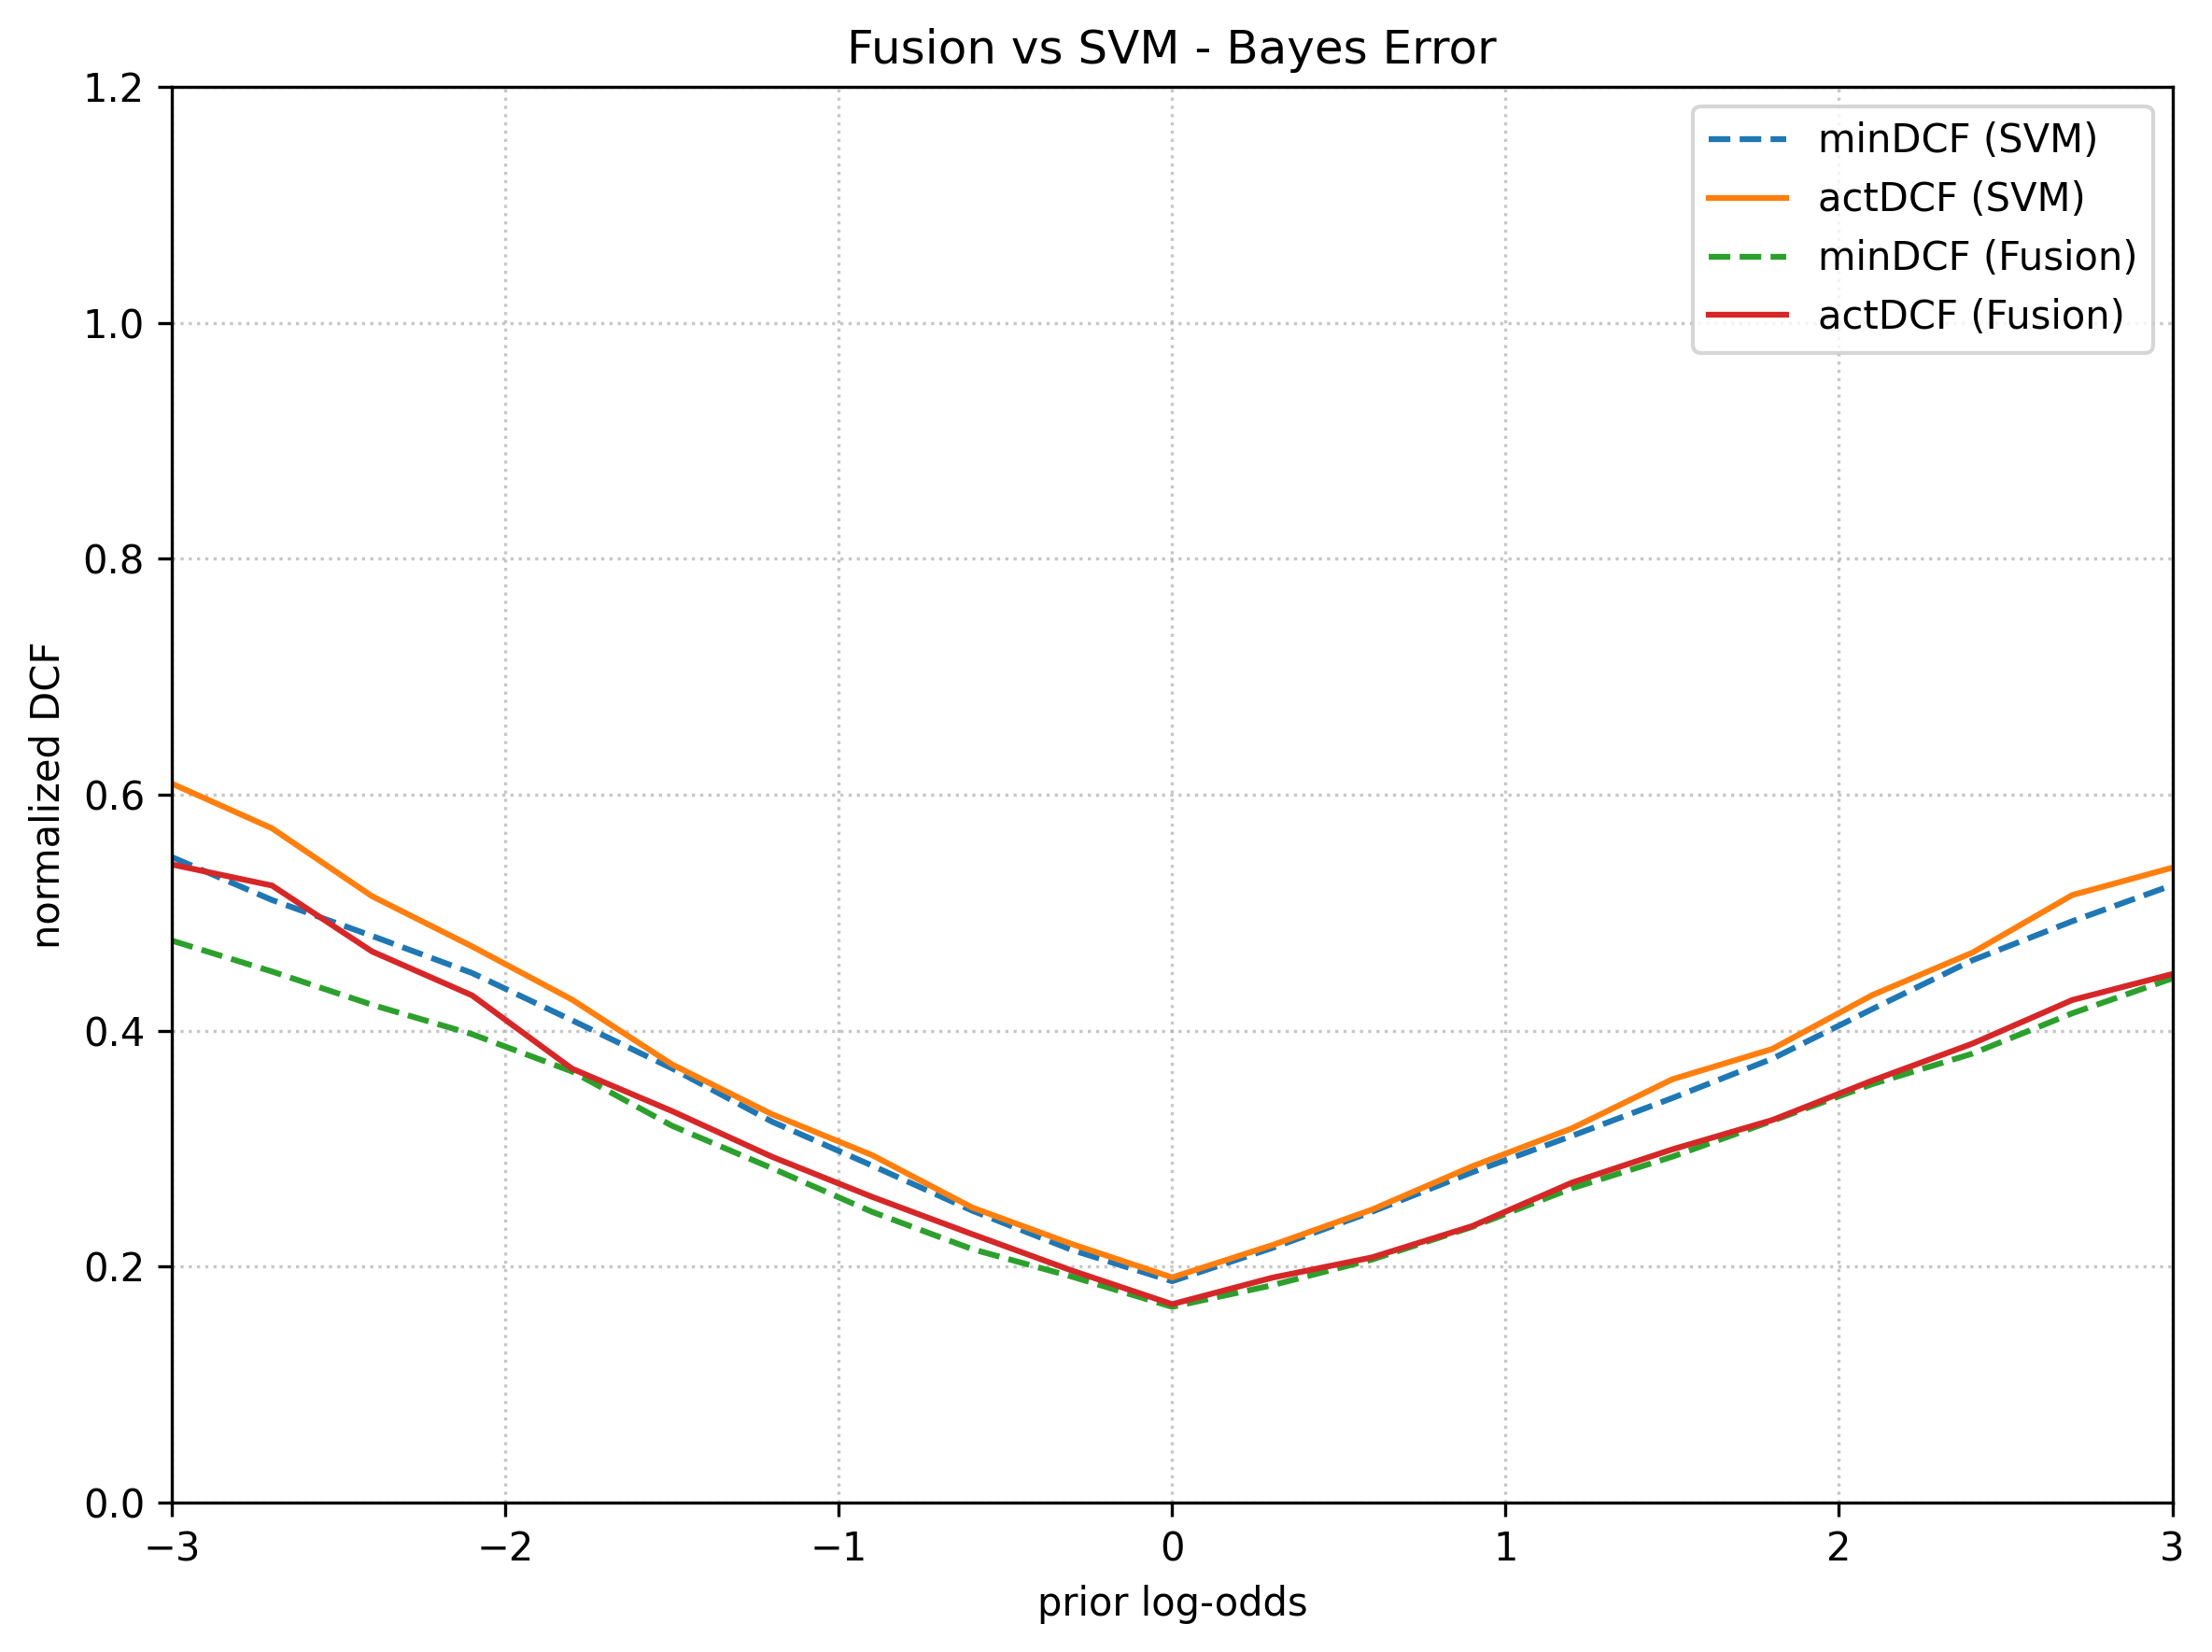
\includegraphics[width=\linewidth]{Bayes_Error_Fusion_vs_SVM.png}
\caption{Bayes Error: Fusion vs. Calibrated SVM.}
\label{fig:fusion_vs_svm}
\end{minipage}\hfill
\begin{minipage}{0.48\textwidth}
\centering
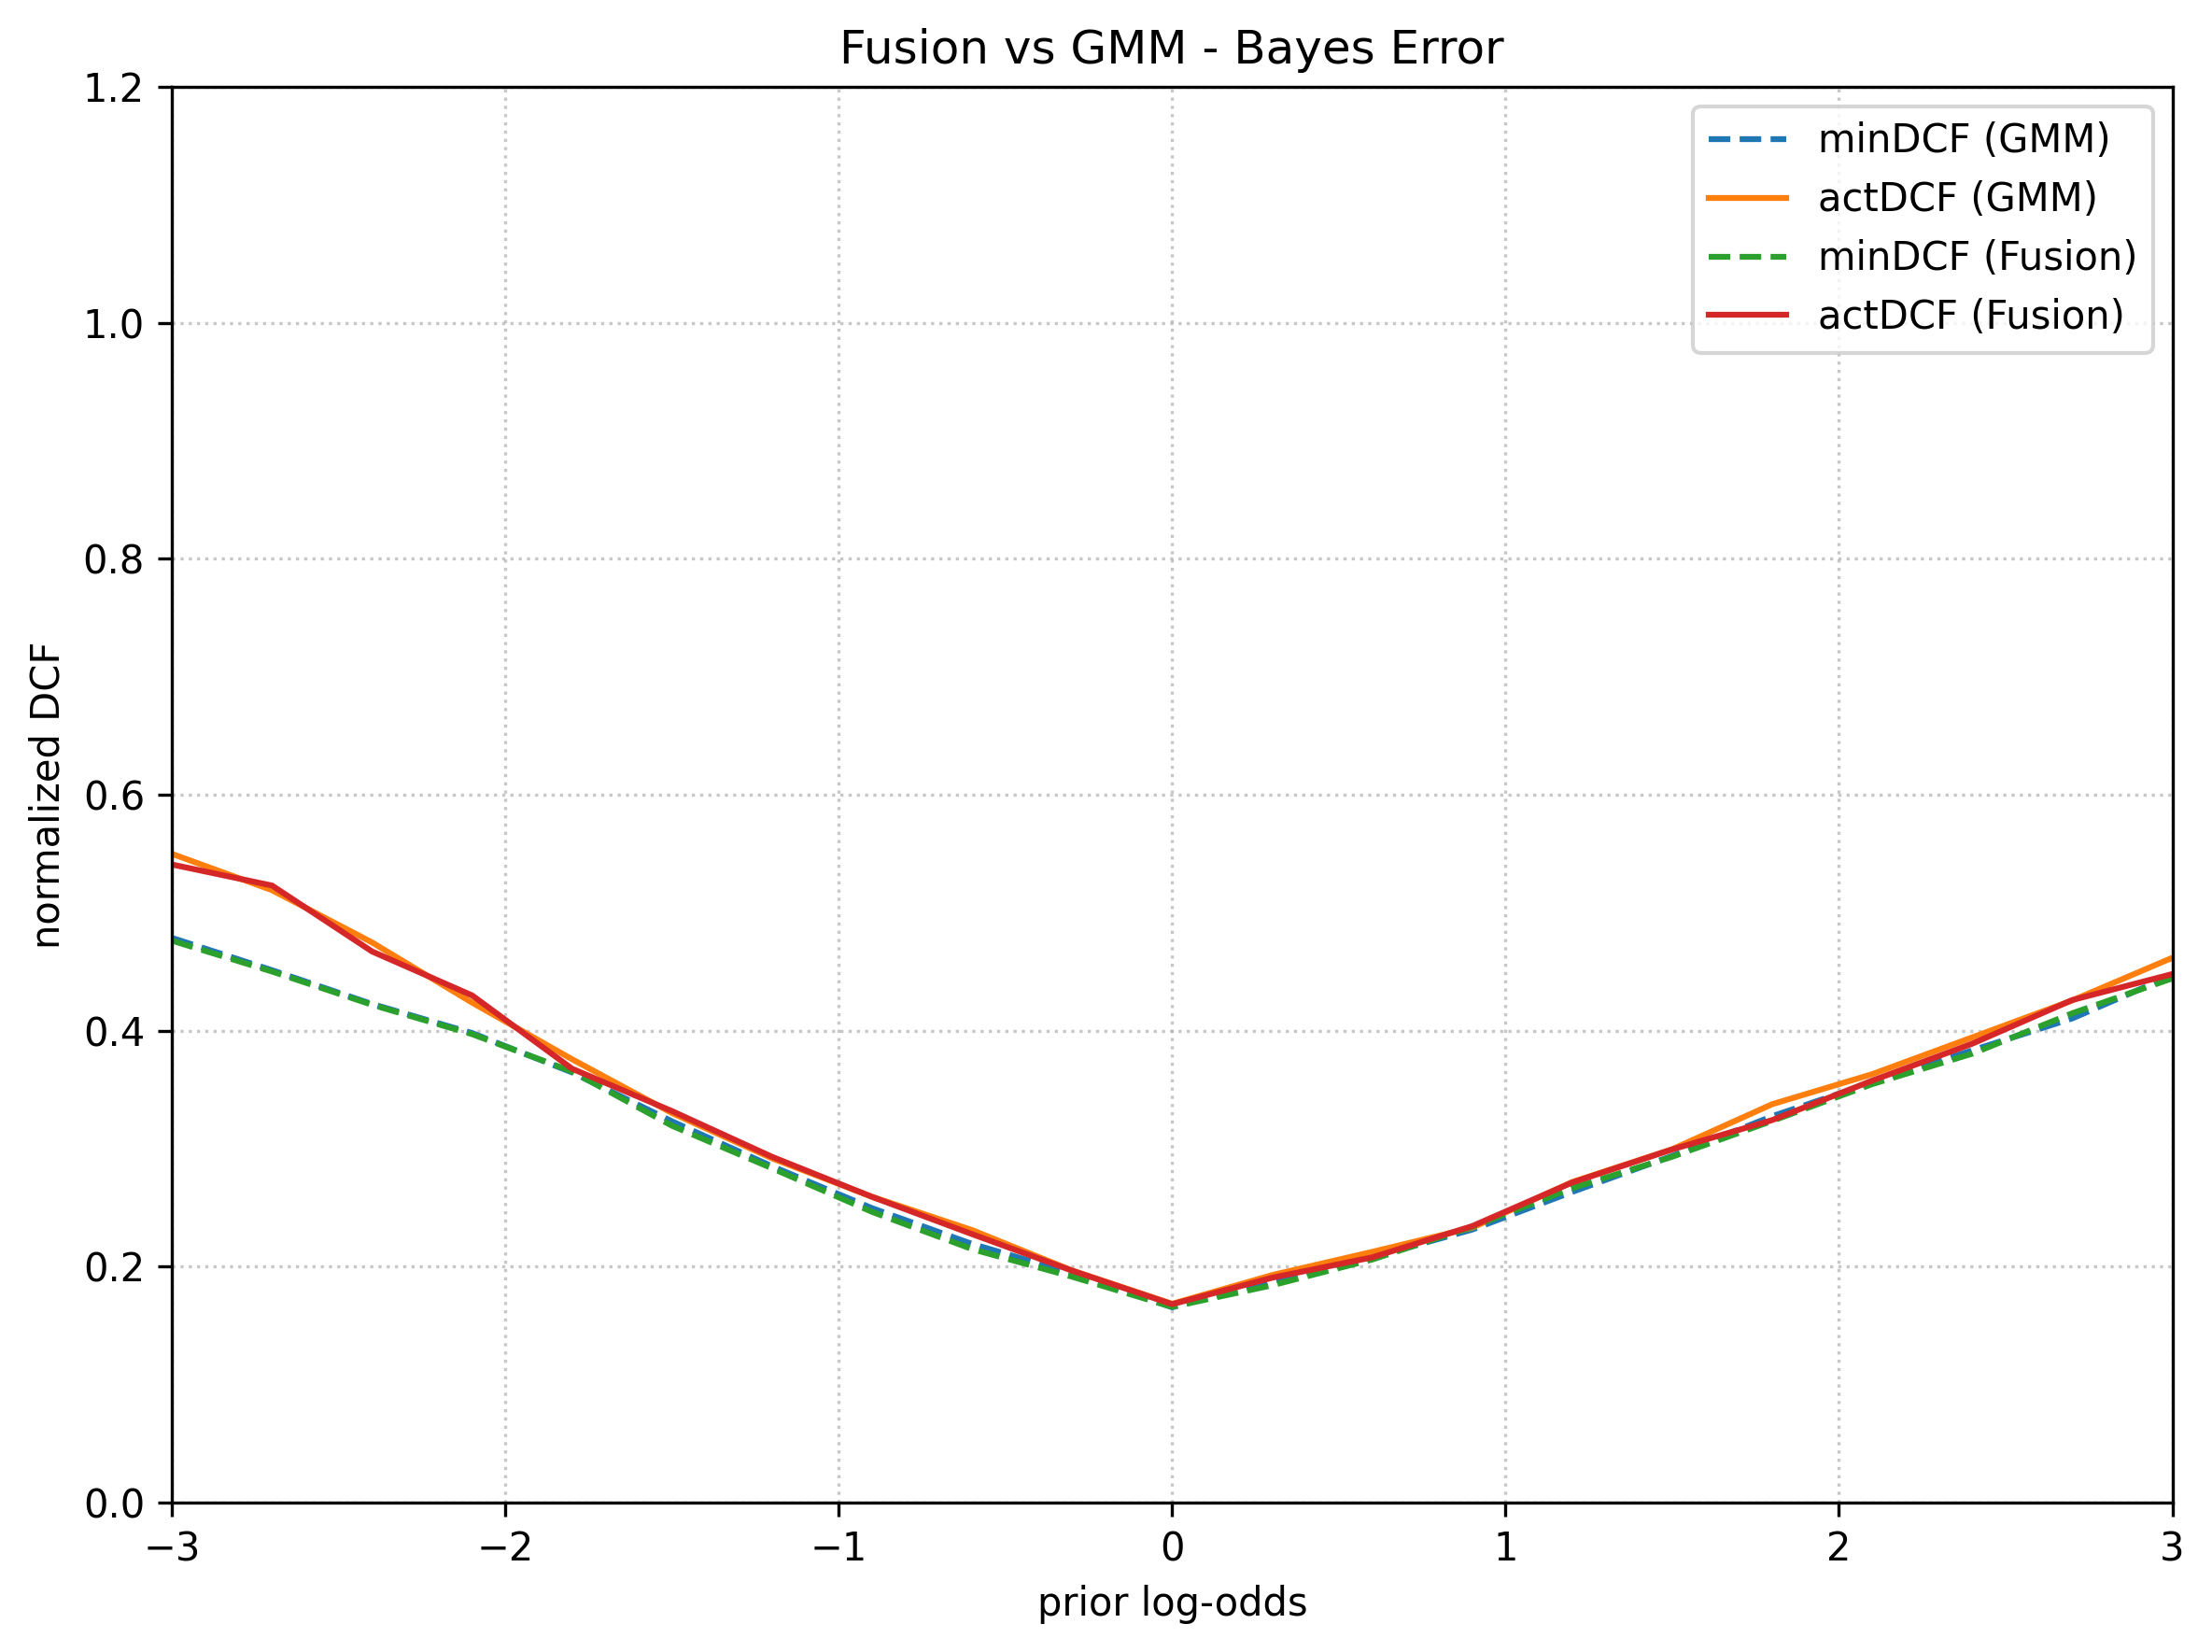
\includegraphics[width=\linewidth]{Bayes_Error_Fusion_vs_GMM.png}
\caption{Bayes Error: Fusion vs. Calibrated GMM.}
\label{fig:fusion_vs_gmm}
\end{minipage}
\end{figure}
\subsection*{Question: What do you observe when comparing the actual DCF error plots?}
Observing the comparative Bayes Error plots, the fused model's Actual DCF curve (red) consistently traces below or perfectly tracks the best available individual curve across the entire log-odds spectrum.
When compared to the SVM (Figure \ref{fig:fusion_vs_svm}), the fusion provides a massive, unmistakable reduction in both Actual and Minimum DCF at all operational points. When compared to the GMM (Figure \ref{fig:fusion_vs_gmm}), the improvement is much narrower, as the GMM is already highly performant. However, the fusion curve still manages to "shave off" the peaks of the GMM's Actual DCF at extreme log-odds, resulting in a system that is slightly more robust and better calibrated than the GMM alone.
\subsection*{Question: Was your final model choice effective?}
Yes, the final model choice (fusing the RBF SVM and the Tied GMM) was highly effective. At every evaluated prior ($\tilde{\pi}=0.1, 0.5, 0.9$), the fused system achieved a lower Minimum DCF than any individual model. For instance, at $\tilde{\pi}=0.9$, the fused system reached a Minimum DCF of \textbf{0.363} (compared to the GMM's 0.365 and SVM's 0.432) and maintained excellent calibration with an Actual DCF of \textbf{0.368}. This mathematically proves that the fusion successfully extracted complementary information from both models.
\subsection*{Question: Would another model/fusion of models have been more effective?}
It is highly unlikely that another combination within our tested architectures would have been more effective. While we could have included Quadratic Logistic Regression in the fusion stack, the results from Chapter 1 demonstrated that it was fundamentally outclassed by both the SVM and GMM in every scenario. Fusing a strictly inferior model (Quadratic LR), which suffers from heavy $L_2$-induced calibration distortion, with highly non-linear and better-calibrated models (RBF SVM, GMM) typically introduces more estimation noise than discriminative value. The pairing of SVM and GMM represents the optimal fusion strategy because they provide the maximum amount of geometric diversity.
\section{Theoretical Considerations}
The success of this Score-Level Fusion is deeply rooted in the concept of \textit{complementary error spaces}. For fusion to be mathematically advantageous, the constituent classifiers must make errors on different regions of the data distribution. Fusing models that fail on the exact same samples yields no improvement.
The RBF SVM and the Tied GMM provide this necessary diversity because they view the feature space through fundamentally opposed mathematical lenses:
\begin{itemize}
\item The \textbf{Tied GMM} is a \textit{generative} model. It assumes the data is generated by a mixture of localized Gaussian clusters and attempts to map the global probability density contours of the entire feature space.
\item The \textbf{RBF Kernel SVM} is a \textit{discriminative} model. It projects data into an infinite-dimensional space to find a strictly local, margin-maximizing boundary. It completely ignores the global density and focuses exclusively on the hardest-to-classify samples (the support vectors) near the boundary edge.
\end{itemize}
Because they utilize completely different geometric assumptions, their "blind spots" rarely overlap. As we observed in Laboratory 4, Features 5 and 6 exhibit heavy skewness with non-Gaussian drop-offs. The GMM, attempting to fit symmetric bells to these skewed tails, will naturally misclassify points lying in the distorted regions of the distribution. Conversely, the SVM makes no Gaussian assumptions; its local RBF kernel can perfectly wrap around those skewed drop-offs, correctly classifying the points the GMM missed.
The fusion Logistic Regression algorithm acts as a linear arbitrator. It learns an optimal plane in the 2D ($s_{\text{SVM}}, s_{\text{GMM}}$) score space, effectively discovering which model to trust in different regions of certainty. By linearly combining these diverse perspectives, the fused boundary becomes a highly robust meta-boundary, mitigating the individual architectural weaknesses of its components and achieving the lowest theoretical error rate on the evaluation set.
\newpage

\chapter{Final System Selection and Conclusion}
\label{chap:conclusion}

Based on the extensive validation and calibration phases conducted in the previous chapters, we select the \textbf{Score-Level Fusion of the RBF Support Vector Machine and the Tied Gaussian Mixture Model} as our final, delivered system. This chapter summarizes the evaluation of this chosen model on the unseen Evaluation dataset and formally addresses the concluding laboratory objectives.

\section{Evaluation of the Delivered System}

\subsection*{Question: Compute minimum and actual DCF, and Bayes error plots for the delivered system. What do you observe? Are scores well calibrated for the target application? And for other possible applications?}

Evaluating our final delivered system (the Fused SVM + GMM) on the unseen Evaluation dataset yields exceptional performance. Across our target applications, the system achieved:
\begin{itemize}
    \item At $\tilde{\pi}=0.1$: Minimum DCF = \textbf{0.406}, Actual DCF = \textbf{0.450}
    \item At $\tilde{\pi}=0.5$: Minimum DCF = \textbf{0.166}, Actual DCF = \textbf{0.168}
    \item At $\tilde{\pi}=0.9$: Minimum DCF = \textbf{0.363}, Actual DCF = \textbf{0.368}
\end{itemize}

Observing these metrics and the corresponding Bayes Error plots (see Figure \ref{fig:fusion_vs_gmm} from Chapter 3), it is evident that the scores are highly well-calibrated for the target applications. The Actual DCF closely tracks the Minimum DCF, particularly at the $\tilde{\pi}=0.5$ and $\tilde{\pi}=0.9$ operational points, where the calibration loss is nearly negligible. 

Furthermore, the scores remain well-calibrated for other possible applications. The Actual DCF curve (red) in the Bayes Error plot remains flat and tightly bounds the Minimum DCF curve (blue) across the entire considered log-odds spectrum from $-4$ to $+4$. This proves that our prior-weighted Logistic Regression fusion strategy successfully projected the raw scores into a globally stable, mathematically sound Log-Likelihood Ratio.

\section{Comparison of Actual DCF and Fusion Effectiveness}

\subsection*{Question: Consider the three best performing systems you selected earlier, and their fusion. Evaluate the corresponding actual DCF, and compare the actual DCF error plots. What do you observe? Was your final model choice effective? Would another model / fusion of models have been more effective?}

Comparing the actual DCF profiles of the calibrated Logistic Regression, SVM, GMM, and the Fused system on the evaluation data, we observe that the Fused system consistently achieves the lowest actual operating cost. For example, at $\tilde{\pi}=0.9$, the fused system reaches an actual DCF of $0.368$, outperforming the calibrated GMM ($0.371$), the calibrated SVM ($0.437$), and the Logistic Regression ($0.462$). 

Our final model choice was highly effective. As observed in the comparative Bayes Error plots, the red actual DCF curve of the fused system consistently sits below the curves of the individual constituent models. 

It is highly unlikely that another fusion combination would have been more effective. The success of our system relies on fusing geometrically complementary models. The RBF SVM provides highly accurate, localized, non-linear margin boundaries, while the Tied GMM provides global, probabilistic density contours. Attempting to fuse a strictly linear, under-performing model like the baseline Logistic Regression into this stack would likely introduce estimation noise without adding any novel discriminative geometric information, ultimately degrading the actual DCF.

\section{Calibration Strategy Effectiveness}

\subsection*{Question: Consider again the three best systems. Evaluate minimum and actual DCF for the target application, and analyze the corresponding Bayes error plots. What do you observe? Was the calibration strategy effective for the different approaches?}

When analyzing the three base systems independently, we observe that the calibration strategy (applying an affine transformation learned via 5-fold cross-validation) was unequivocally effective, though the magnitude of the improvement varied depending on the model's native architecture:

\begin{enumerate}
    \item \textbf{Support Vector Machine:} The strategy was overwhelmingly effective. Because SVMs naturally output unbounded geometric margin distances rather than probabilities, the raw scores were catastrophically miscalibrated at extreme priors (e.g., raw actual DCF of $0.631$ at $\tilde{\pi}=0.1$). Calibration successfully mapped these distances into true LLRs, dropping the actual DCF to $0.347$ on the validation set and stabilizing the Bayes Error plot.
    \item \textbf{Logistic Regression:} The strategy was highly effective at correcting the bias introduced by the model's initial training parameters. The calibration successfully shifted the threshold to align with the target applications, closing the gap between the actual and minimum DCF curves at the extremes.
    \item \textbf{Gaussian Mixture Model:} The strategy was effective, though less drastic. Because the GMM natively computes probabilistic likelihoods, its baseline calibration was already strong. However, the calibrator successfully compensated for minor density distortions caused by the non-Gaussian skewed tails in the dataset, further refining the actual DCF across all target applications.
\end{enumerate}

In conclusion, score calibration and geometrically diverse score-level fusion are indispensable steps for deploying generative and discriminative pattern recognition systems in real-world, highly asymmetric target applications.
\end{document}
